\newpage
\maketitle
\begin{center}
\Large \textbf{第4章 协整模型} \quad 
\end{center}
\begin{abstract}
在本章中我们将首先讲述交易对的概念,并讲述如何利用交易对的均值回归特性,通过对交易对的多空操作,实现稳定的盈利。在本章中,我们主要讲解交易对的数学原理,怎样确定对冲比例。对于怎样利用交易对进行统计套利策略研发,将在后续章节中介绍。
\end{abstract}
\section{协整模型}
本章讲述的内容是统计套利策略,这是一种市场中性策略,无论是市场是涨是跌,均有可能盈利。将统计套利用到极致的例子,应该属于上世纪90年代的LTCM基金。LTCM基金成立于1994年,成立时基金规模为12.5亿美金,但是到1997年,基金规模就达到了48亿美金,是当时世界上四大基金之一。LTCM基金的创始人是金牌交易员,合伙人是顶级统计学家,他们发现德国国债和意大利国债有一个稳定的比例关系,大概率波动的机率会非常小,因此当德国国债上涨时,德国国债与意大利国债之比将增大,大幅度偏离均值,他们就卖出德国国债,买入意大利国债,一段时间之后,德国国债会下跌,德国国债和意大利国债之比就会回归到均值,此时他们卖出之前买入的意大利国债,重新买入之前卖出的德国国债,这样他们持有德国国债和意大利国债没有发生变化,但是却赚到了这次波动差价所产生的利润。利用这种方式,LTCM基金获得了巨大的成功。然而LTCM基金的神话终结于1997年,主要有以下几个原因:首先LTCM认为德国国债和意大利国债之比符合正态分布,但是虽然自然界大部分复杂的现象都是正态分布,但是人类社会现象,却不一定是正态分布,黑天鹅事件也许是长态,在1997年,东南亚发生了金融危机,俄罗斯发生了国债违约,正是这两个黑天鹅事件,使德国国债与意大利国债之比不再符合正态分布,而LTCM基金由于对这些事件缺乏预见性,而遭受了巨大的损失;同时,在LTCM基金破产之后,人们看LTCM基金的财务数据发现,其资金杠杆高达数万倍,因此一次失误的决策,就足以使整个公司破产。由这个实例我们可以看出,基于交易对均值回归的统计回归策略,具有巨大的盈利潜力,同时我们也应看到,杠杆是魔鬼,任何策略中最重要的都是资金和仓位管理。\newline
交易对不仅在传统金融市场,如股市、期货、外汇、债市上存在,在新兴的加密货币市场,也是一种非常重要的策略,前一两年兴起的比特币搬砖模式,就是交易对策略在加密货市场的应用。
\subsection{数据模拟}
\subsubsection{协整模型构建}
根据\cite{r000002}的内容,我们可以通过模拟数据来加深我们对基本概念的理解。假设$\{ w_{t} \}$为白噪声,在此基础上定义随机游走信号:
\begin{equation}
z_{t} = z_{t-1} + w_{t}
\label{e000058}
\end{equation}
在此基础上我们定义两个非平稳的时间序列信号:
\begin{equation}
x_{t} = pz_{t} + w_{t} = 0.3z_{t} + w_{t}
\label{e000059}
\end{equation}
\begin{equation}
y_{t} = qz_{t} + w_{t} = 0.6z_{t} + w_{t}
\label{e000060}
\end{equation}
如果我们将$\{ x_{t} \}$和$\{ y_{t} \}$进行线性组合:
\begin{equation}
ax_{t} + by_{t} = (ap+bq)z_{t} + w_{t} = (0.3a+0.6b)z_{t} + w_{t}
\label{e000061}
\end{equation}
如果$0.3a+0.6b=0$的话,那么$\{ x_{t} \}$和$\{ y_{t} \}$的这个线性组合就只剩下白噪声信号,因此其是
平稳时间序列信号,因此当$a=2, b=-1$时,这个序列就是平稳时间序列信号。\newline
根据这一思想,程序如下所示:
\lstset{language=PYTHON, caption={线性组合形成平稳时间序列}, label={c000010}}
\begin{lstlisting}
    def simulate_demo(self):
        '''
        模拟数据生成
        '''
        # 生成白噪声信号
        samples = 1000
        w = np.random.standard_normal(size=samples)
        # 生成随机游走序列
        z = np.zeros((samples,))
        for t in range(1, samples):
            z[t] = z[t-1] + w[t]
        # 生成非平稳信号,即交易对x和y
        x = np.zeros((samples,))
        y = np.zeros((samples,))
        p = 0.3
        q = 0.6
        for t in range(samples):
            x[t] = p*z[t] + w[t]
            y[t] = q*z[t] + w[t]
        fig = plt.figure(figsize=(6, 6))
        w_plt = plt.subplot(2, 2, 1, title='White Noise: w')
        w_plt.plot(w)
        z_plt = plt.subplot(2, 2, 2, title='Random Walk: z')
        z_plt.plot(z)
        x_plt = plt.subplot(2, 2, 3, title='Non Stationary Signal: x')
        x_plt.plot(x)
        y_plt = plt.subplot(2, 2, 4, title='Non Stationary Signal: y')
        y_plt.plot(y)
        fig.tight_layout()
        plt.show()
        # 生成协整信号
        a = 2
        b = -1
        c = a * x + b * y
        plt.plot(c)
        plt.title('Cointegration Model')
        plt.show()
        # 采用ADF检验 
        resid_adf = unitroot.ADF(c)
        print('stat={0:0.4f} vs 1%_cv={1:0.4f}'.format( \
                    resid_adf.stat, resid_adf.critical_values['1%']))
        if resid_adf.stat < resid_adf.critical_values['1%']:
            print('resid为稳定时间序列 ^_^')
        else:
            print('resid为非稳定时间序列!!!!!')
\end{lstlisting}
我们首先绘制出白噪声、随机游走和x及y信号:
\begin{figure}[H]
	\caption{研究序列}
	\label{f000042}
	\centering
	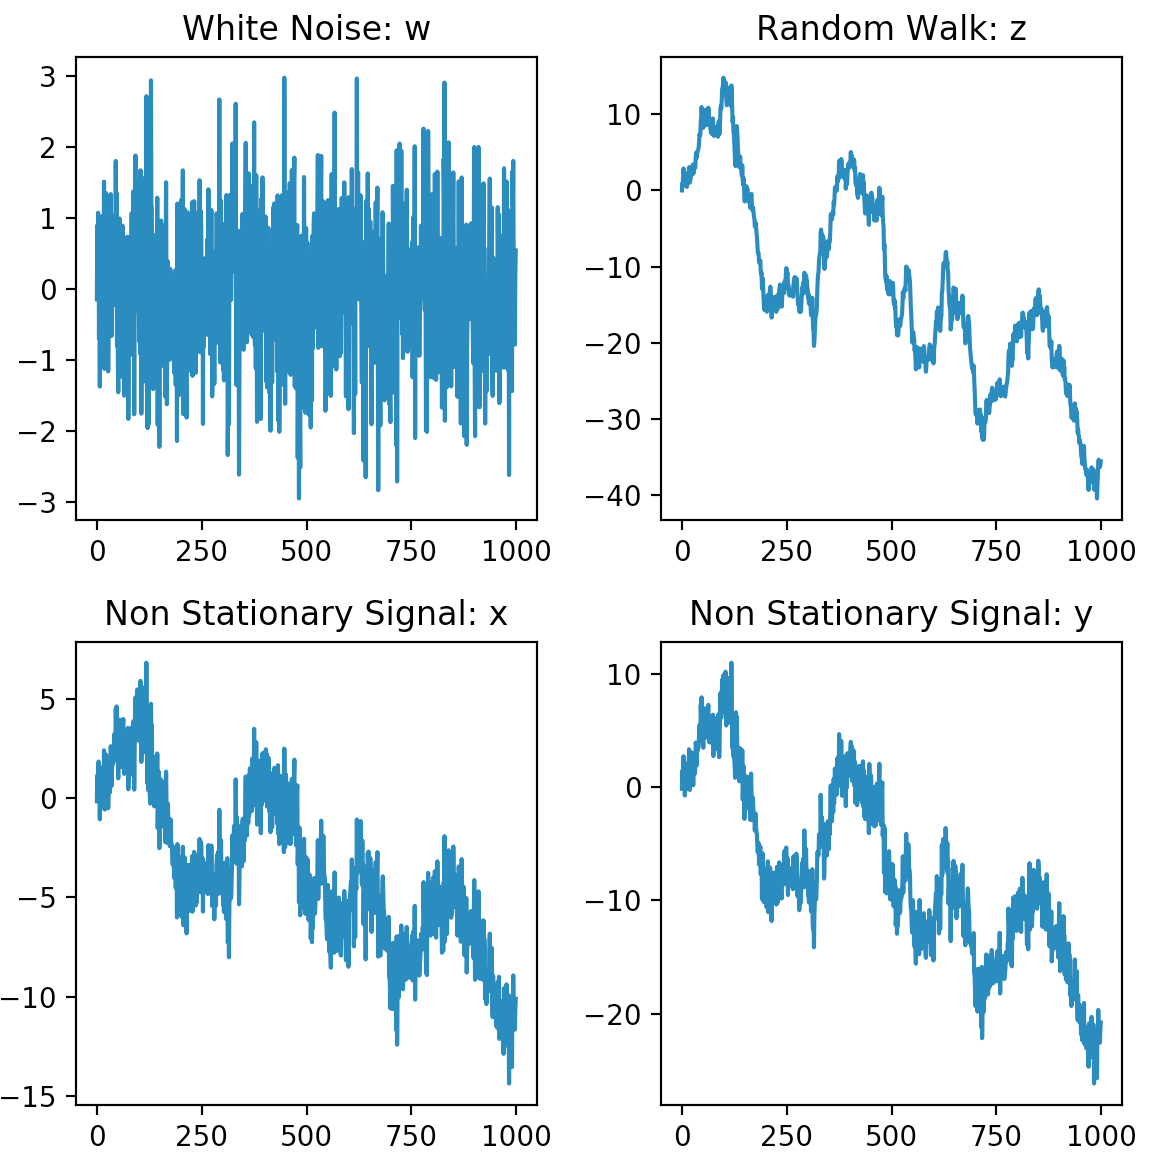
\includegraphics[height=5cm]{images/f000042}
\end{figure}
接着我们绘制出x和y的线性组合:
\begin{figure}[H]
	\caption{x和y的线性组合}
	\label{f000043}
	\centering
	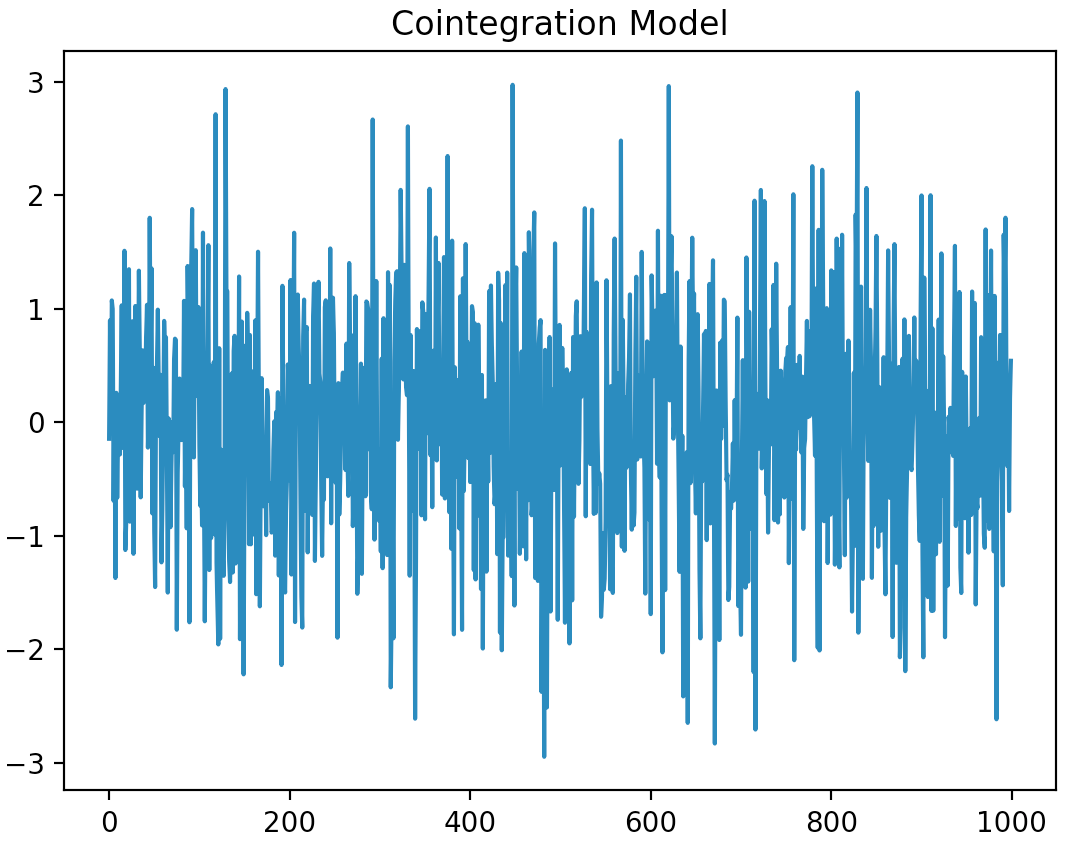
\includegraphics[height=5cm]{images/f000043}
\end{figure}
我们利用ADF检验其稳写性:
\begin{figure}[H]
	\caption{ADF检验}
	\label{f000044}
	\centering
	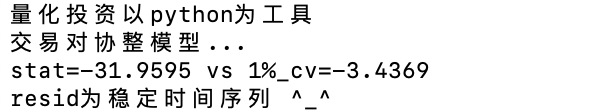
\includegraphics[height=1cm]{images/f000044}
\end{figure}
由上面的ADF检验可以看出,x和y的线性组合与理论分析一致,是平稳时间序列。
\subsubsection{对冲比例确定}
在上面的例子中,我们验证了我们的假设,即对两个非平稳的时间序列进行线性组合,通过选择合适的系数,可以得到平稳时间序
列信号。现在的问题就变为怎样求出这些系数,使线性组合后的时间序列具有平稳性。在这一节中,我们将向大家演示采用线性
回归技术,来求出线性组合的系数。虽然线性回归算法非常简单,尤其是我们这里只有一维,就更简单了。但是这里我们将采用
Google在今年3月新推出的TensorFlow 2.0 alpha,采用高级API keras来完成这一过程。\newline
\paragraph{线性回归模型}
在讲解确定线性组合系数之前,我们先来讲解一下为达到这一目的所开发的基于TensorFlow 2.0的线性回归模型。代码如下所示:
\lstset{language=PYTHON, caption={基于TensorFlow 2.0的线性回归模型}, label={c000011}}
\begin{lstlisting}
    import numpy as np
    import matplotlib.pyplot as plt
    import tensorflow as tf
    
    class QciLinearRegression(object):
        def __init__(self, train_x=None, train_y=None, 
                    validate_x=None, validate_y=None, 
                    test_x=None, test_y=None):
            self.name = 'QciLinearRegression'
            self.loss = 'mean_squared_error'
            self.learning_rate = 0.01
            self.optimizer = tf.keras.optimizers.Adam(self.learning_rate)
            self.epoch = 50000
            if train_x:
                self.train_x = train_x
                self.train_y = train_y
                self.validate_x = validate_x
                self.validate_y = validate_y
                self.test_x = test_x
                self.test_y = test_y
            else:
                self.train_x, self.train_y, self.validate_x, \
                            self.validate_y, self.test_x, \
                            self.test_y = self.generate_dataset()
    
        def generate_dataset(self):
            train_x = np.array([-40, -10, 0, 8, 15, 22, 38, 20, 9, 13], dtype=float)
            train_y = np.array([-40, 14, 32, 46, 59, 72, 100, 68, 48.2, 55.4], dtype=float)
            validate_x = np.array([], dtype=float)
            validate_y = np.array([], dtype=float)
            test_x = np.array([], dtype=float)
            test_y = np.array([], dtype=float)
            return train_x, train_y, validate_x, validate_y, test_x, test_y
    
        def train(self):
            model = self.build_model()
            model.compile(loss=self.loss, optimizer=self.optimizer)
            class PrintDot(tf.keras.callbacks.Callback):
                def on_epoch_end(self, epoch, logs):
                    if epoch % 100 == 0: print('')
                    print('epoch:{0}...{1}!'.format(epoch, logs))
            early_stop = tf.keras.callbacks.EarlyStopping(monitor='val_loss', patience=10)
            history = model.fit(self.train_x, self.train_y, 
                        epochs=self.epoch, validation_split = 0.1,  
                        verbose=False, callbacks=[early_stop, PrintDot()])
            plt.title('linear regression training process')
            plt.xlabel('epochs')
            plt.ylabel('error')
            plt.plot(history.history['loss'])
            plt.show()
            model.save('./work/aqt003_qiclr')
            weights = np.array(model.get_weights())
            print(weights)
    
        def build_model(self):
            layer1 = tf.keras.layers.Dense(units=1, input_shape=[1])
            model = tf.keras.Sequential([layer1])
            return model
    
        def predict(self, data):
            model = tf.keras.models.load_model('./work/aqt003_qiclr')
            rst = model.predict(data)
            return rst
    
    if '__main__' == __name__:
        lr = QciLinearRegression()
        lr.train()    
\end{lstlisting}
初始化函数的参数为训练样本集、验证样本集和测试样本集,缺省值为空,当不传递这些值时,我们采用类内定义的
generate\_dataset方法来为这些属性赋值。同时,在构造函数中设定了代价函数为最小平方误差函数,学习率为0.01,优化
算法为最常用的Adam,训练遍数为5万。\newline
在generate\_dataset函数中,我们输入特征为摄氏度的温度,而输出值为华氏度的温度,二者的关系为:
\begin{equation}
F = 1.8 \times C + 32
\label{e000062}
\end{equation}
我们任务就是学出1.8和32这两个参数。\newline
外部程序通过调用train方法作为入口,程序首先调用build\_model方法生成模型,我们的这个网络由两层组成,第1层为输入层
只有一个节点,第2层为输出层,其也只有一个节点,这个网络的参数为:第1层节点到第2层节点的连接权值和第2层神经元的偏置
值。创建完模型之后,我们通过model.compile来设置模型的代价函数和优化算法;为了提高模型的泛化能力避免overfitting,
我们采用early stopping算法,当验证集上的精度在10个循环中没有明显改进时,停止训练过程(在后面的日志中,我们可以看到
虽然我们定义训练5万次,但是实际训练不到1万次就停止了)。接着我们定义一个临时类,因为神经网络训练
通常会很耗时,我们用这个函数打印当前进度情况。接着我们调用model.fit来开始实际训练过程,在后台日志中我们可以看到,误差
会逐渐减少,如图所示:
\begin{figure}[H]
	\caption{程序运行日志}
	\label{f000045}
	\centering
	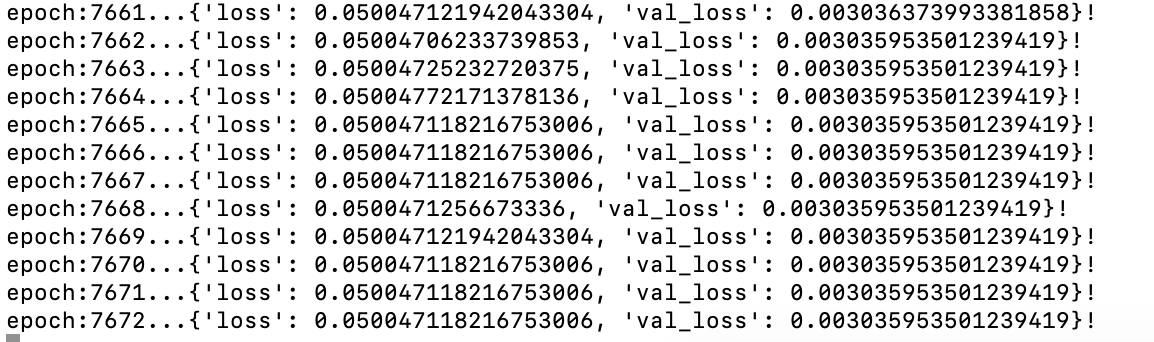
\includegraphics[height=3cm]{images/f000045}
\end{figure}
我们可以看到最后一列的验证集上的误差在10次没有明显变化时,由于early stopping算法,训练过程就自动结束了。接下来我们
可以绘制出误差随训练时间的变化过程,如下所示:
\begin{figure}[H]
	\caption{误差变化曲线}
	\label{f000046}
	\centering
	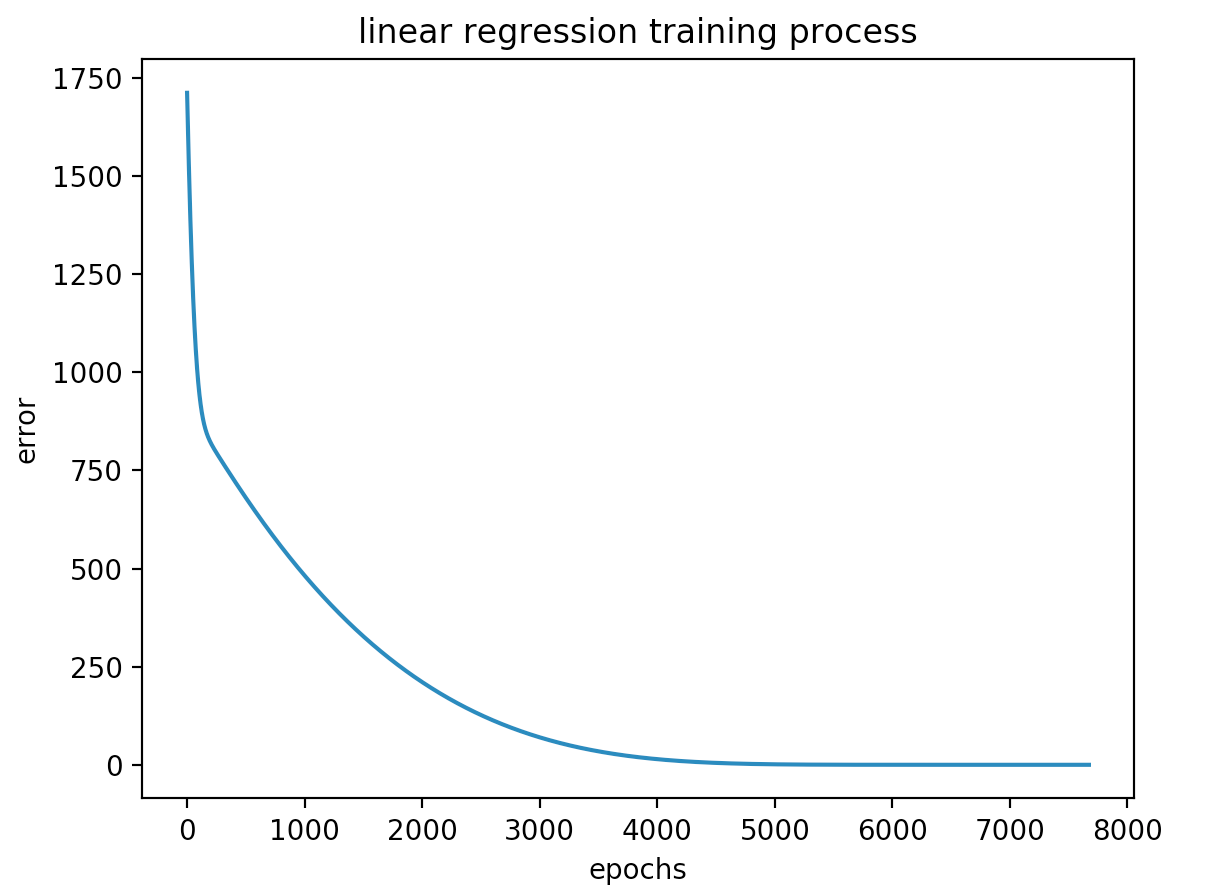
\includegraphics[height=1cm]{images/f000046}
\end{figure}
最终学到的参数值为:
\begin{figure}[H]
	\caption{误差变化曲线}
	\label{f000047}
	\centering
	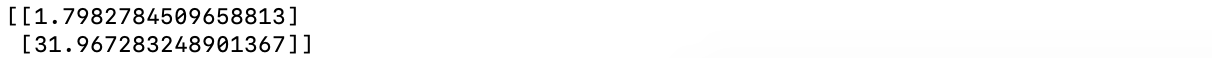
\includegraphics[height=1cm]{images/f000047}
\end{figure}
我们看到其与实际值就非常接近了,证明我们线性回归模型是正确的。虽然在我们协整模型中用不到,但是我们还是介绍一下当网络训
练完成之后,下一步就给出数据,让其给我们算出真实的结果,这在predict方法中实现。在predict方法中,首先从模型文件中
恢复出网络结构,然后运行模型的predict方法生成并返回预测值,调用代码如下所示:
\lstset{language=PYTHON, caption={利用线性回归模型进行预测}, label={c000012}}
\begin{lstlisting}
    data = np.array([[100.0]], dtype=float)
    rst = qcilr.predict(data)
    print(rst)
\end{lstlisting}
运行结果如下所示:
\begin{figure}[H]
	\caption{预测值}
	\label{f000048}
	\centering
	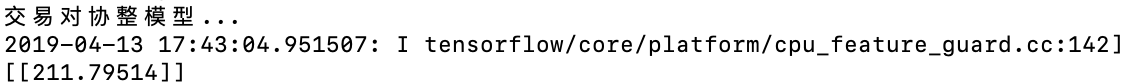
\includegraphics[height=1cm]{images/f000048}
\end{figure}
\paragraph{对冲比例确定}
在有了线性回归模型之后,下面我们就用线性回归模型来确定对冲比例。程序如下所示:
\lstset{language=PYTHON, caption={线性回归模型确定对冲比例}, label={c000013}}
\begin{lstlisting}
    def qcilr_demo(self):
        # 生成白噪声信号
        samples = 1000
        w = np.random.standard_normal(size=samples)
        # 生成随机游走序列
        z = np.zeros((samples,))
        for t in range(1, samples):
            z[t] = z[t-1] + w[t]
        # 生成非平稳信号,即交易对x和y
        x = np.zeros((samples,))
        y = np.zeros((samples,))
        p = 0.3
        q = 0.6
        for t in range(samples):
            x[t] = p*z[t] + w[t]
            y[t] = q*z[t] + w[t]
        fig = plt.figure(figsize=(6, 6))
        w_plt = plt.subplot(2, 2, 1, title='White Noise: w')
        w_plt.plot(w)
        z_plt = plt.subplot(2, 2, 2, title='Random Walk: z')
        z_plt.plot(z)
        x_plt = plt.subplot(2, 2, 3, title='Non Stationary Signal: x')
        x_plt.plot(x)
        y_plt = plt.subplot(2, 2, 4, title='Non Stationary Signal: y')
        y_plt.plot(y)
        fig.tight_layout()
        plt.show()
        # 以x作为自变量
        w1, x_y_p = self.do_linear_regression(x, y)
        # 将y作为自变量
        w2, y_x_p = self.do_linear_regression(y, x)
        print('xToy={0}({1}) vs yTox={2}({3})'.format(x_y_p, w1[0][0], y_x_p, w2[0][0]))
        if x_y_p < y_x_p:
            print('######## x  为自变量')
            c = w1[0][0] * x - y
        else:
            print('######### y  为自变量')
            c = w2[0][0] * y - x
        plt.title('Final Cointegration Signal')
        plt.plot(c)
        plt.show()
\end{lstlisting}
在上面的程序中,我们首先像上一节一样,先做出x和y两个非平稳的时间序列信号,然后我们先以x为自变量做一次线性回归,
求出ADF检验的p值和对冲比例,再以y作为自变量做一次线性回归,求出ADF检验的值p和对冲比例,我们取ADF检验的p值较小的
一个作为最终结果,求出线性组合的信号c,最后绘制出其信号典线。\newline
原始信号如下所示:
\begin{figure}[H]
	\caption{原始信号}
	\label{f000049}
	\centering
	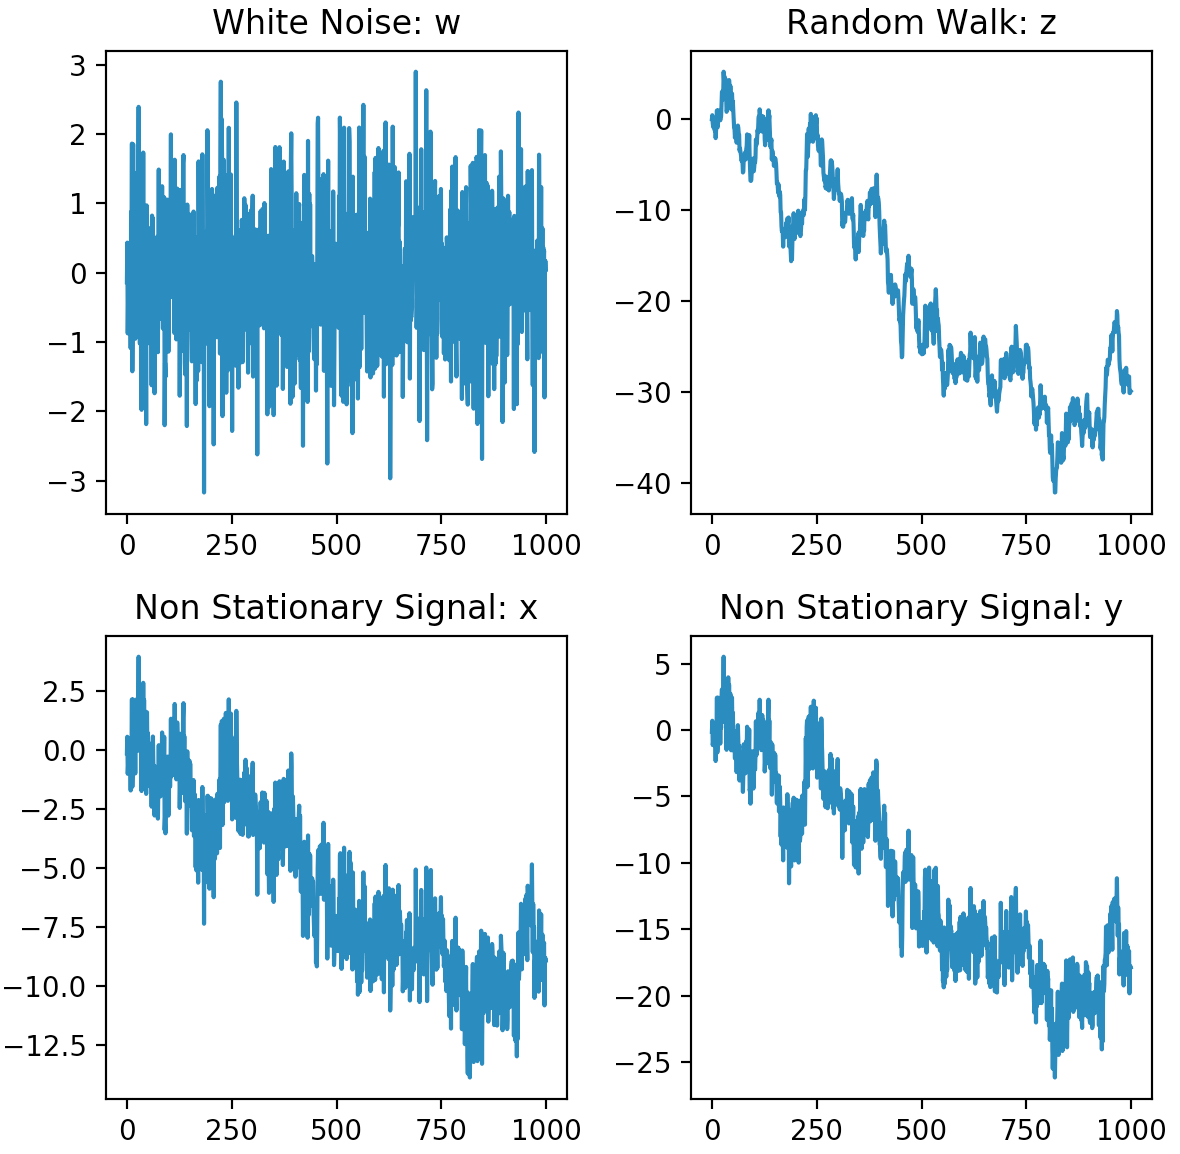
\includegraphics[height=5cm]{images/f000049}
\end{figure}
以x为自变量时线性回归运行情况:
\begin{figure}[H]
	\caption{以x为自变量的线性回归}
	\label{f000050}
	\centering
	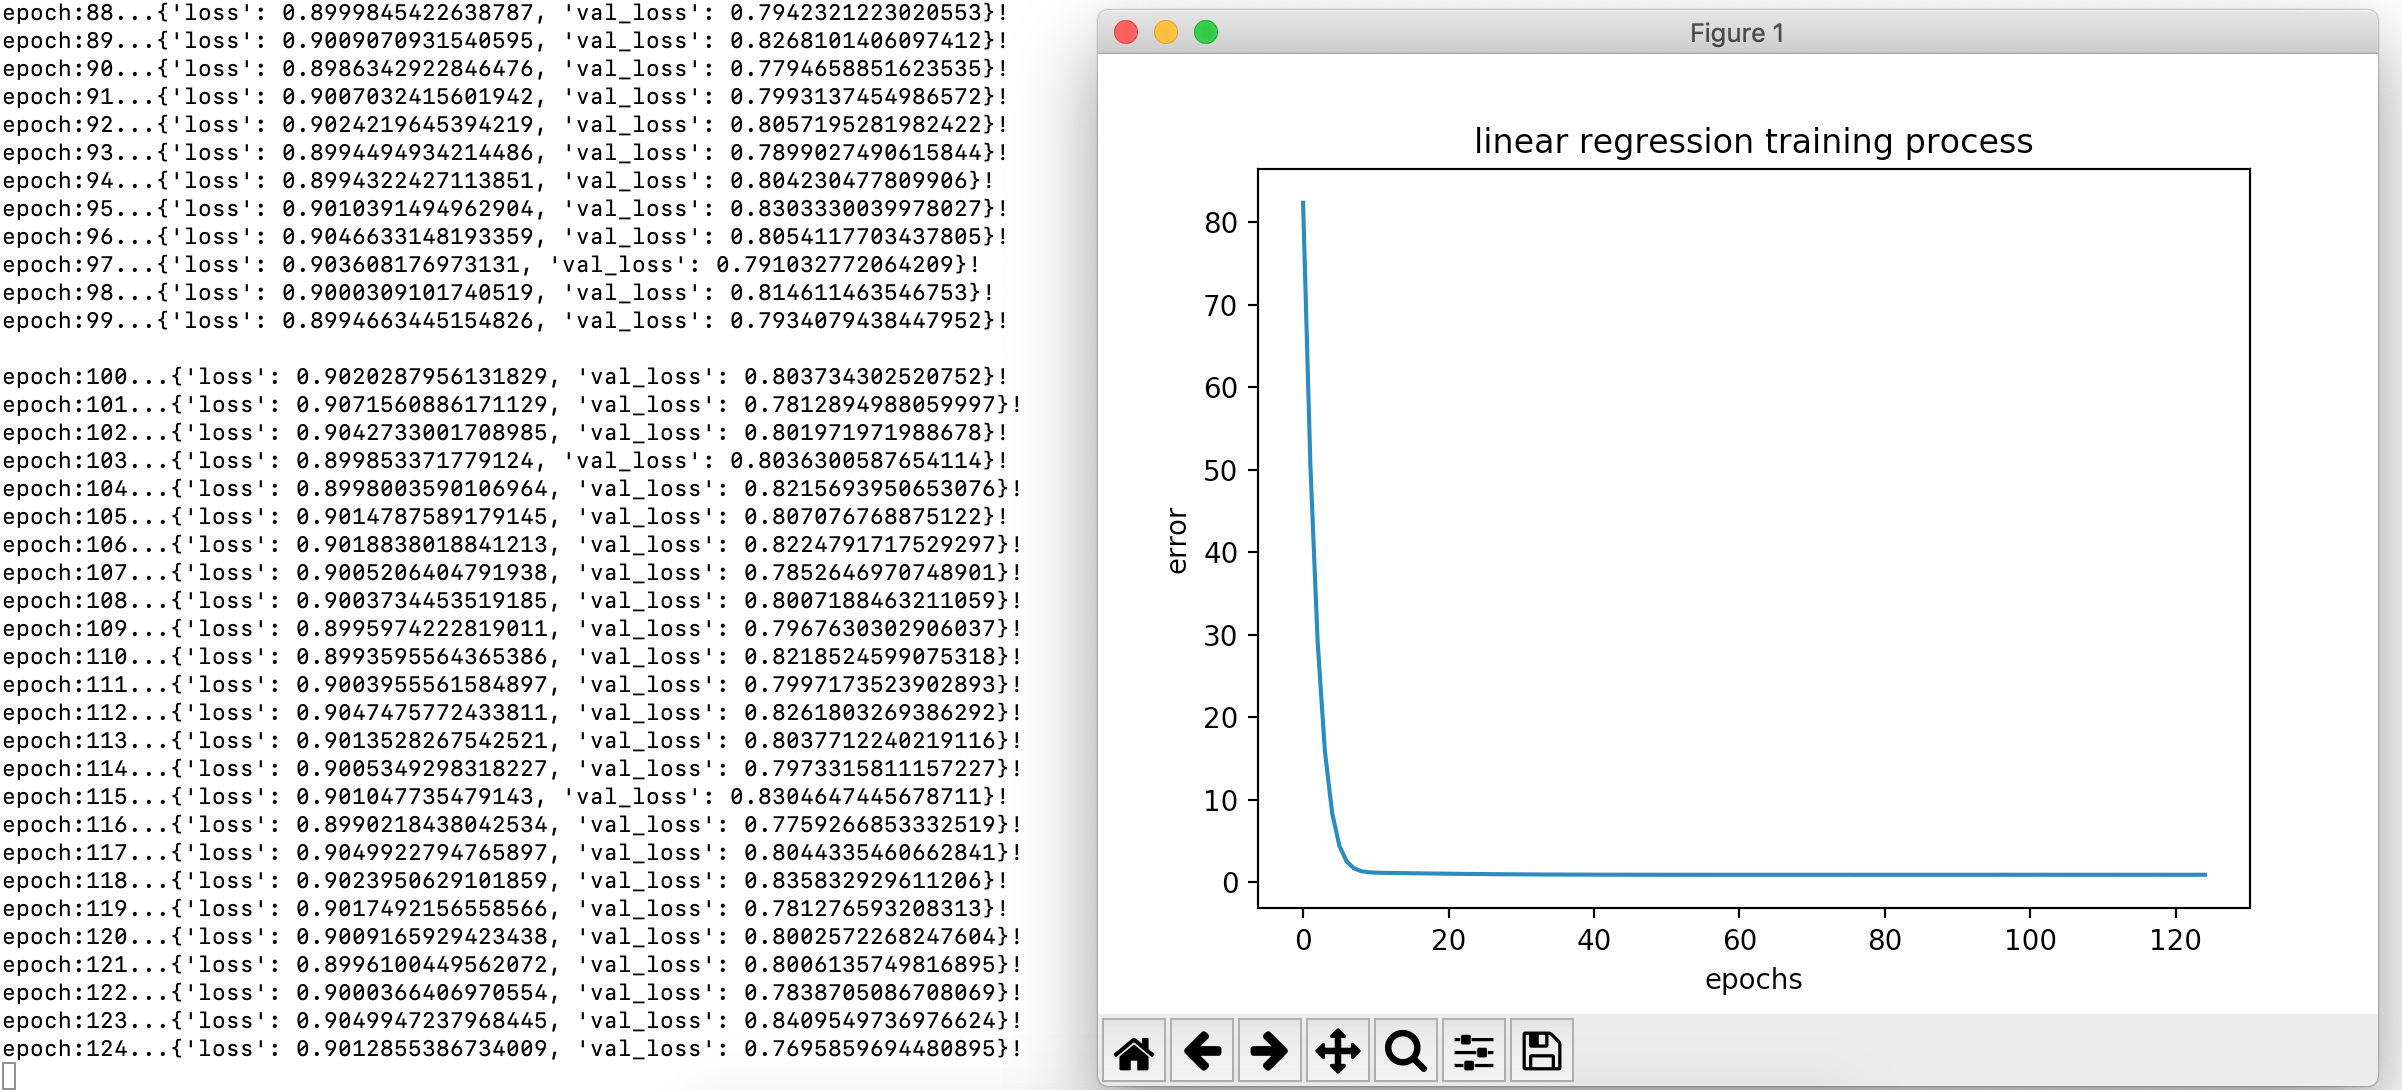
\includegraphics[height=5cm]{images/f000050}
\end{figure}
以y为自变量时线性回归运行情况:
\begin{figure}[H]
	\caption{以y为自变量时线性回归}
	\label{f000051}
	\centering
	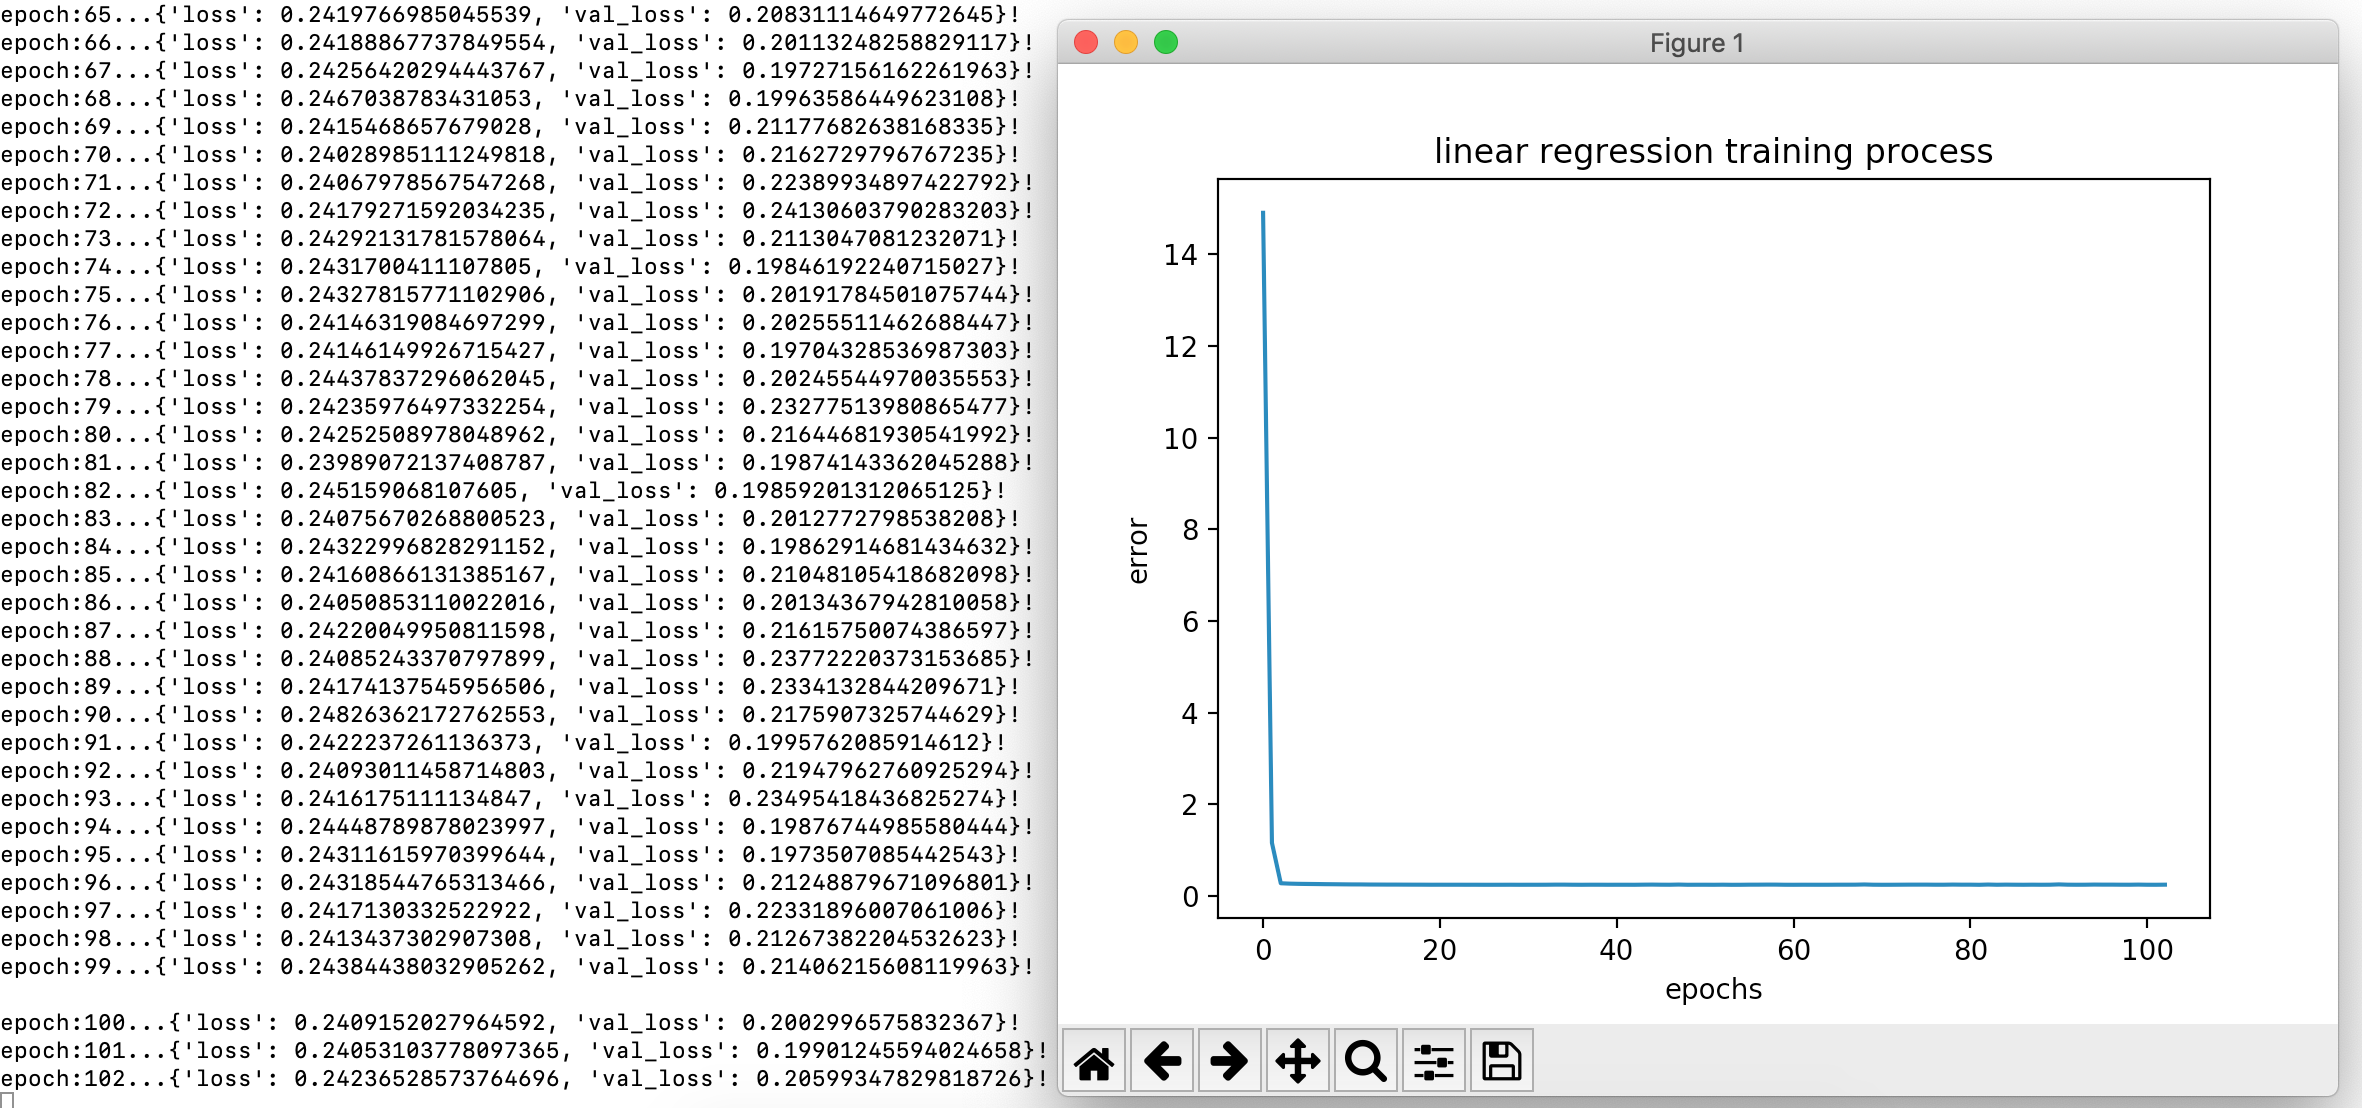
\includegraphics[height=5cm]{images/f000051}
\end{figure}
最后的协整信号结果:
\begin{figure}[H]
	\caption{协整信号}
	\label{f000052}
	\centering
	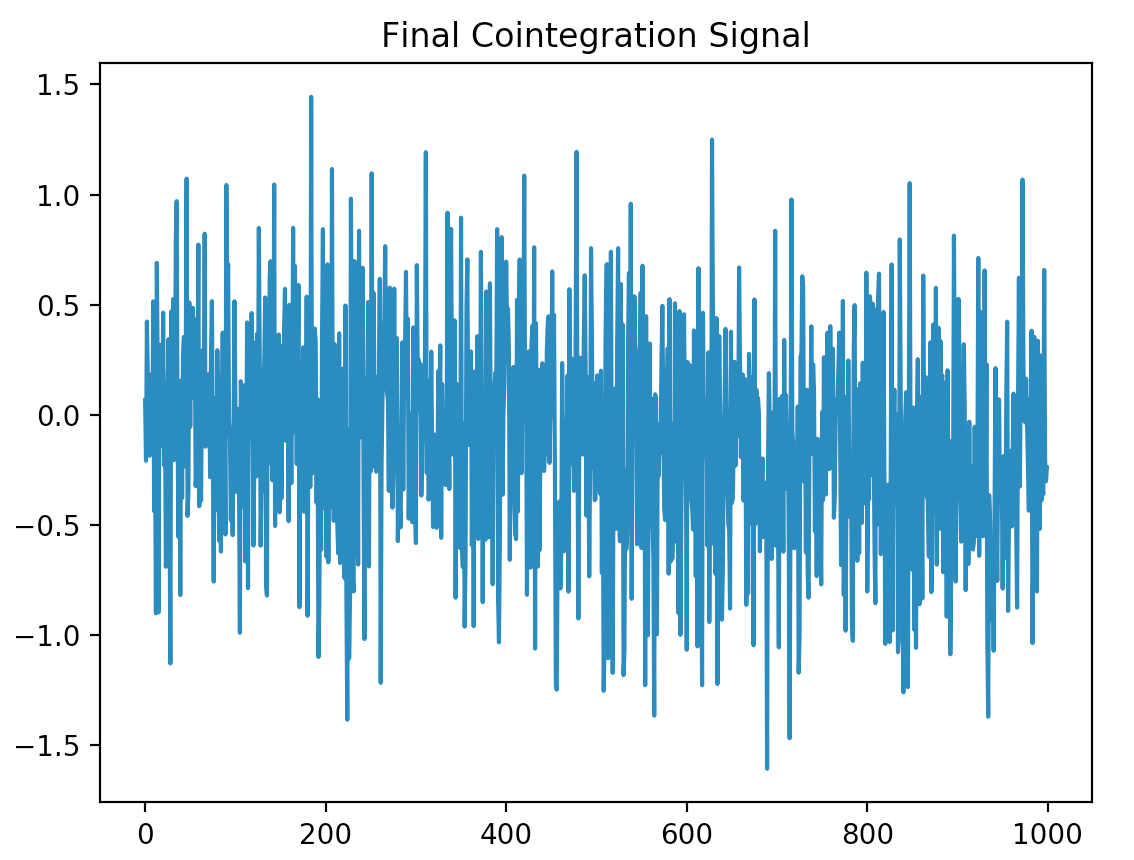
\includegraphics[height=5cm]{images/f000052}
\end{figure}
程序的运行结果如下所示:
\begin{figure}[H]
	\caption{程序运行结果}
	\label{f000053}
	\centering
	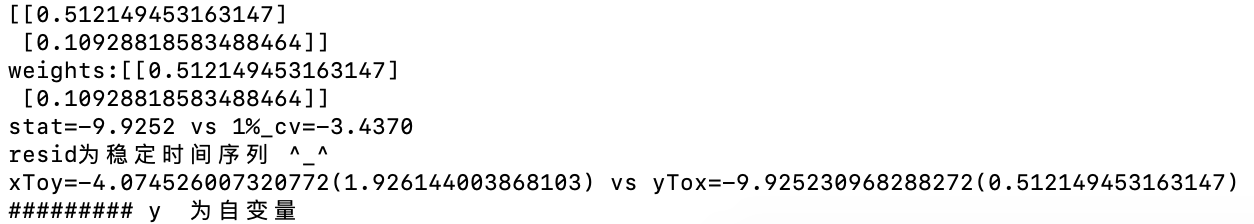
\includegraphics[height=5cm]{images/f000053}
\end{figure}
由于以y为自变量时ADF检验的p值较小,所以取以y为自变量的情况,计算出来的对冲比例为0.51,与实际值0.5非常接近,
这证明我们的算法是正确的。
\subsection{Johansen检验}
我们已经讲述了协整模型理论,可以比较好的处理两个交易对的对冲比例和均值回归的问题。但是这里面有两个问题,首先在协整模
型中,我们假设交易对中的两个标的是线性关系,其次我们只能处理有两个标的的交易对。在本节中,我们将根据\cite{r000001}
投资组合理论,处理标的之间不是线性关系,以及多个交易标的的均值回归策略研发问题。\newline
在实际应用中,我们经常用到的模型是Johansen Test模型,有时也叫VECM模型。在这一节中,我们将来讲解这个模型。Johansen模
型是基于向量自回归VAR模型的。我们以前所讲的自回归模型,都是标量的自回归模型,向量自回归模型定义为:
\begin{equation}
\boldsymbol{x}_{t} = \boldsymbol{\mu} + A_{1}\boldsymbol{x}_{t-1} + ... + A_{p}\boldsymbol{x}_{t-p} + \boldsymbol{w}_{t}
\label{e000063}
\end{equation}
式中$\symbol{\mu}$为序列的均值向量,$\boldsymbol{w}_t$为白噪声向量。接下来我们定义向量误差修正模块VECM(Vector Error Correction Model):
\begin{equation}
\Delta \boldsymbol{x}_{t}= \boldsymbol{\mu} + A \boldsymbol{x}_{t-1} + \Gamma _{1} \Delta \boldsymbol{x}_{t-1} + ... + \Gamma _{p} \Delta \boldsymbol{x}_{t-p} + \boldsymbol{w}_t
\label{e000064}
\end{equation}
其中A为系数矩阵,$\Gamma _{i}$是各滞后期的系数矩阵。我们对矩阵A进行特征值分解,阶数为$r$,分为以下两种情况:
\begin{itemize}
\item $r=0$:表明没有线性协整模型;
\item $r>0$:至少有$r+1$个序列存在协整关系;
\end{itemize}
在实际应用中,我们取出最大的特征值对应的特征向量,将其元素作为对应序列的协整系数。